\documentclass[aspectratio=169]{beamer}
\usepackage[utf8]{inputenc}
\usepackage[T5]{fontenc}
\usepackage[vietnamese]{babel}
\usepackage{graphicx}
\usepackage{hyperref}
\usepackage{lmodern}

% Theme
\usetheme{Madrid}
\usecolortheme{whale}

% Metadata
\title[Hệ Khuyến nghị Cây trồng]{Ứng dụng AI trong Nông nghiệp}
\subtitle{Chương 5: Hệ khuyến nghị cây trồng (Crop Recommender)}
\author{Giảng viên}
\institute{Đại học Đông Á}
\date{\today}

\begin{document}

\begin{frame}
    \titlepage
\end{frame}

\begin{frame}{Nội dung chính}
    \tableofcontents
\end{frame}

\section{Giới thiệu \& Đặt vấn đề}
\begin{frame}{Thách thức trong Nông nghiệp hiện đại}
    \begin{itemize}
        \item Nông nghiệp là ngành kinh tế chính, nhưng năng suất vẫn chưa tối ưu do:
        \begin{itemize}
            \item Lựa chọn cây trồng sai lầm dựa trên trực giác truyền thống.
            \item Quản lý đồng ruộng và vật nuôi kém hiệu quả.
            \item Biến đổi khí hậu, hiện tượng nóng lên toàn cầu làm thời tiết khó đoán.
        \end{itemize}
        \item Hậu quả: Năng suất giảm, thu nhập của nông dân giảm sút nghiêm trọng.
        \item \textbf{Giải pháp:} Cần áp dụng công nghệ để phân tích các thông số khí hậu và đất đai nhằm đưa ra quyết định canh tác chính xác.
    \end{itemize}
\end{frame}

\begin{frame}{Hệ khuyến nghị cây trồng bằng Học máy (Machine Learning)}
    \begin{itemize}
        \item \textbf{Mục tiêu:} Đề xuất loại cây trồng phù hợp nhất cho từng vùng đất, giúp tối đa hóa năng suất.
        \item \textbf{Đầu vào (Features):}
        \begin{itemize}
            \item Các thành phần của đất: Nitơ (N), Phốt pho (P), Kali (K), độ pH.
            \item Yếu tố môi trường: Nhiệt độ, Độ ẩm, Lượng mưa.
        \end{itemize}
        \item \textbf{Đầu ra (Target):} 22 loại cây trồng (Ngô, bông, lúa, cà phê, dừa, táo, xoài,...).
    \end{itemize}
\end{frame}

\section{Các nghiên cứu liên quan}
\begin{frame}{Tổng quan các nghiên cứu đã thực hiện}
    Nhiều nghiên cứu trước đây đã áp dụng Machine Learning vào phân loại cây trồng:
    \begin{itemize}
        \item \textbf{Doshi và cộng sự (2018):} Dùng Cây quyết định (DT), Rừng ngẫu nhiên (RF), Mạng nơ-ron (NN), KNN để dự đoán sự phù hợp với nhiệt độ, lượng mưa, đất.
        \item \textbf{Kumar và cộng sự (2015):} Dùng SVM, RF, KNN dựa trên mật độ nước và đất.
        \item \textbf{Shakil và cộng sự (2015):} Áp dụng Hồi quy tuyến tính, ANN, và KNN để dự đoán cho các loại ngũ cốc.
        \item $\rightarrow$ Hầu hết các thuật toán học có giám sát đều mang lại độ chính xác cao khi có dữ liệu đầu vào tốt.
    \end{itemize}
\end{frame}

\section{Quy trình thực nghiệm}
\begin{frame}{Sơ đồ quy trình thực nghiệm}
    \begin{columns}
        \begin{column}{0.4\textwidth}
            \begin{itemize}
                \item Thu thập và hợp nhất các bộ dữ liệu.
                \item Trực quan hóa để tìm ra mối tương quan.
                \item Làm sạch (Tiền xử lý) dữ liệu.
                \item Xây dựng và đánh giá các mô hình học máy.
            \end{itemize}
        \end{column}
        \begin{column}{0.6\textwidth}
            \begin{center}
                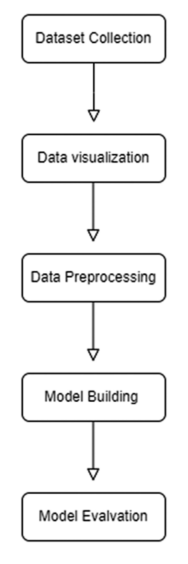
\includegraphics[width=0.95\textwidth,height=0.65\textheight,keepaspectratio]{chap5_img_3_0.png}
                
                \vspace{0.2cm}
                \textit{Hình 5.1: Sơ đồ các bước thực nghiệm}
            \end{center}
        \end{column}
    \end{columns}
\end{frame}

\section{Trực quan hóa dữ liệu}
\begin{frame}{Trực quan hóa: Yêu cầu về lượng mưa}
    \begin{columns}
        \begin{column}{0.4\textwidth}
            \begin{itemize}
                \item Biểu đồ cột (Bar chart) giúp xác định lượng mưa trung bình cần thiết cho từng loại cây trồng.
                \item Việc phân tích đơn biến giúp đưa ra các quyết định lựa chọn cây trồng sơ bộ.
            \end{itemize}
        \end{column}
        \begin{column}{0.6\textwidth}
            \begin{center}
                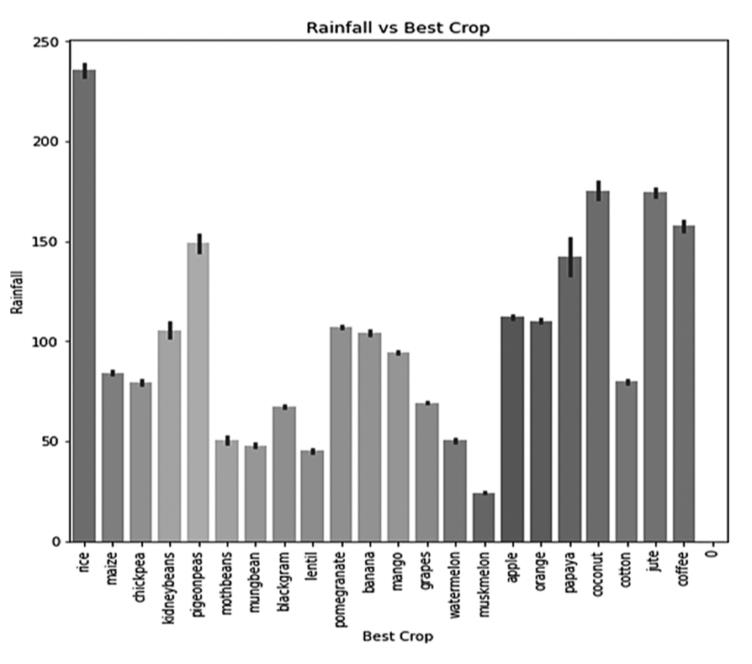
\includegraphics[width=0.95\textwidth,height=0.65\textheight,keepaspectratio]{chap5_img_4_0.png}
                
                \vspace{0.2cm}
                \textit{Hình 5.2: Yêu cầu lượng mưa cho các loại cây trồng}
            \end{center}
        \end{column}
    \end{columns}
\end{frame}

\begin{frame}{Trực quan hóa: Ma trận tương quan (Heatmap)}
    \begin{columns}
        \begin{column}{0.4\textwidth}
            \begin{itemize}
                \item Phân tích đa biến bằng Heatmap giúp thấy được mối quan hệ giữa các đặc trưng (N, P, K, Nhiệt độ...).
                \item \textbf{Tương quan dương:} Ví dụ giữa Phốt pho (P) và Kali (K).
                \item \textbf{Tương quan âm:} Giữa P và lượng mưa, độ pH.
            \end{itemize}
        \end{column}
        \begin{column}{0.6\textwidth}
            \begin{center}
                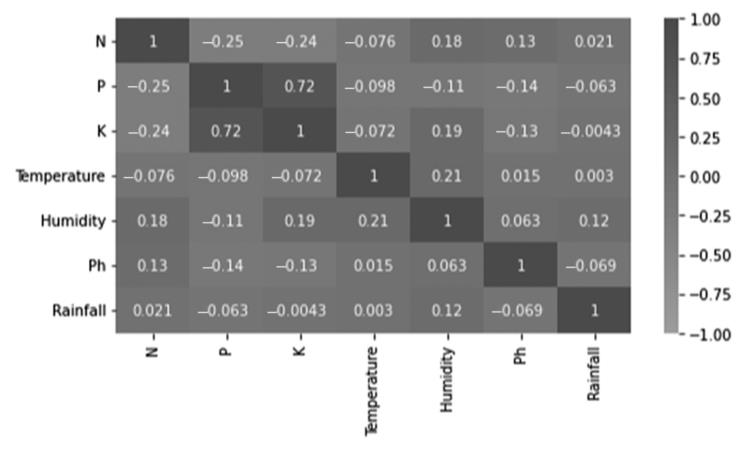
\includegraphics[width=0.95\textwidth,height=0.65\textheight,keepaspectratio]{chap5_img_5_0.png}
                
                \vspace{0.2cm}
                \textit{Hình 5.3: Biểu đồ nhiệt tương quan giữa các đặc trưng}
            \end{center}
        \end{column}
    \end{columns}
\end{frame}

\section{Tiền xử lý dữ liệu}
\begin{frame}{Làm sạch và Tiền xử lý dữ liệu}
    Làm sạch dữ liệu là bước bắt buộc để mô hình học máy đạt độ chính xác cao:
    \begin{itemize}
        \item \textbf{Loại bỏ nhiễu và ngoại lai (Outliers):} 
        \begin{itemize}
            \item Lỗi nhập liệu, dữ liệu không nhất quán sẽ làm sai lệch mô hình.
            \item Nghiên cứu sử dụng khoảng tứ phân vị (IQR) để phát hiện và kỹ thuật giới hạn (Capping) để xử lý ngoại lai.
        \end{itemize}
        \item \textbf{Co giãn đặc trưng (Feature Scaling):}
        \begin{itemize}
            \item Đưa tất cả các biến (pH nhỏ (1-14), Lượng mưa lớn (hàng trăm mm)) về cùng một thang đo.
            \item Giúp mô hình không bị thiên vị (bias) đối với các đặc trưng có giá trị số lớn.
        \end{itemize}
    \end{itemize}
\end{frame}

\section{Xây dựng mô hình và Đánh giá}
\begin{frame}{Xây dựng hệ khuyến nghị (Bagging \& Ensemble)}
    \begin{itemize}
        \item Dữ liệu sau khi làm sạch (70\% Huấn luyện, 30\% Kiểm tra) được đưa vào các thuật toán phân loại.
        \item Nghiên cứu sử dụng phương pháp \textbf{Bagging} (Bootstrap Aggregating) và tập hợp (Ensemble).
        \item Ensemble kết hợp nhiều mô hình cơ sở yếu để tạo ra một mô hình dự đoán mạnh và đáng tin cậy hơn.
        \item Việc so sánh giữa các bộ phân loại đơn lẻ (DT, SVM) và các phương pháp tập hợp (RF, Bagging) cho thấy phương pháp tập hợp tối ưu hơn cho bài toán hệ khuyến nghị.
    \end{itemize}
\end{frame}

\begin{frame}{Mô hình: Cây quyết định (Cơ sở \& Thuật toán)}
    \begin{columns}
        \begin{column}{0.4\textwidth}
            \begin{itemize}
                \item Cây quyết định (Decision Tree) chia nhỏ dữ liệu dựa trên thuộc tính có Lợi ích thông tin (Information Gain) cao nhất.
                \item Dễ hiểu, dễ giải thích và hoạt động như cách con người đưa ra quyết định.
            \end{itemize}
        \end{column}
        \begin{column}{0.6\textwidth}
            \begin{center}
                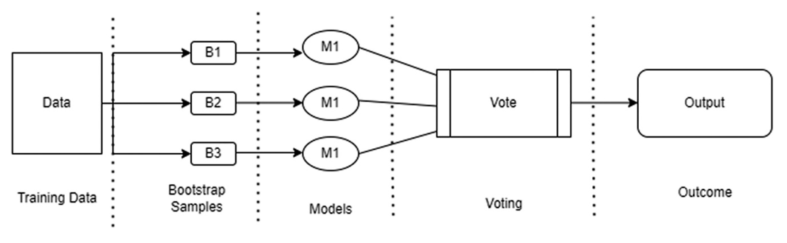
\includegraphics[width=0.95\textwidth,height=0.65\textheight,keepaspectratio]{chap5_img_7_0.png}
                
                \vspace{0.2cm}
                \textit{Minh họa thuật toán / cơ sở toán học}
            \end{center}
        \end{column}
    \end{columns}
\end{frame}

\begin{frame}{Sơ đồ Cây quyết định}
    \begin{columns}
        \begin{column}{0.4\textwidth}
            \begin{itemize}
                \item Cấu trúc gồm: Nút gốc (Root), Nút quyết định (Decision) và Nút lá (Terminal).
                \item Mỗi nhánh đại diện cho một kịch bản hoặc một điều kiện phân chia.
            \end{itemize}
        \end{column}
        \begin{column}{0.6\textwidth}
            \begin{center}
                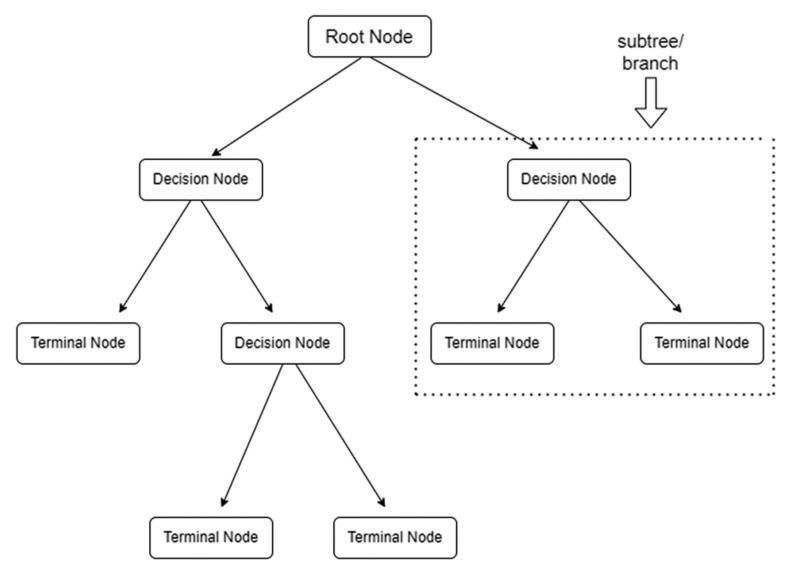
\includegraphics[width=0.95\textwidth,height=0.65\textheight,keepaspectratio]{chap5_img_8_0.png}
                
                \vspace{0.2cm}
                \textit{Hình 5.5: Sơ đồ cấu trúc Cây quyết định}
            \end{center}
        \end{column}
    \end{columns}
\end{frame}

\begin{frame}{Mô hình: Mạng nơ-ron (Neural Network)}
    \begin{columns}
        \begin{column}{0.4\textwidth}
            \begin{itemize}
                \item Mạng nơ-ron nhân tạo (ANN) gồm các lớp: Đầu vào (Input), Ẩn (Hidden), Đầu ra (Output).
                \item MLP (Multi-Layer Perceptron) xử lý tốt các bộ dữ liệu phi tuyến tính phức tạp.
            \end{itemize}
        \end{column}
        \begin{column}{0.6\textwidth}
            \begin{center}
                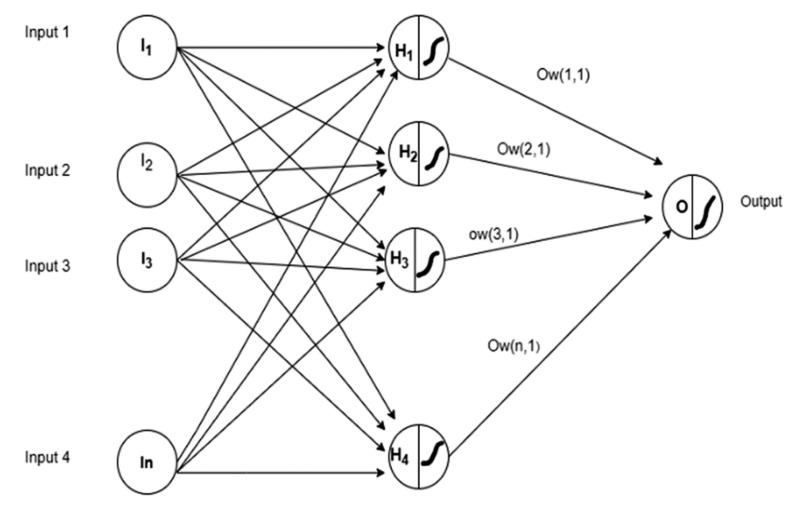
\includegraphics[width=0.95\textwidth,height=0.65\textheight,keepaspectratio]{chap5_img_9_0.png}
                
                \vspace{0.2cm}
                \textit{Hình 5.6: Sơ đồ một mạng nơ-ron}
            \end{center}
        \end{column}
    \end{columns}
\end{frame}

\begin{frame}{Đánh giá mô hình: Đường cong AUROC}
    \begin{columns}
        \begin{column}{0.4\textwidth}
            \begin{itemize}
                \item AUROC đo lường khả năng phân biệt tín hiệu so với nhiễu (TPR so với FPR).
                \item Giá trị tối ưu nằm ở góc trên bên trái; mô hình đạt AUROC lên đến 0.998.
            \end{itemize}
        \end{column}
        \begin{column}{0.6\textwidth}
            \begin{center}
                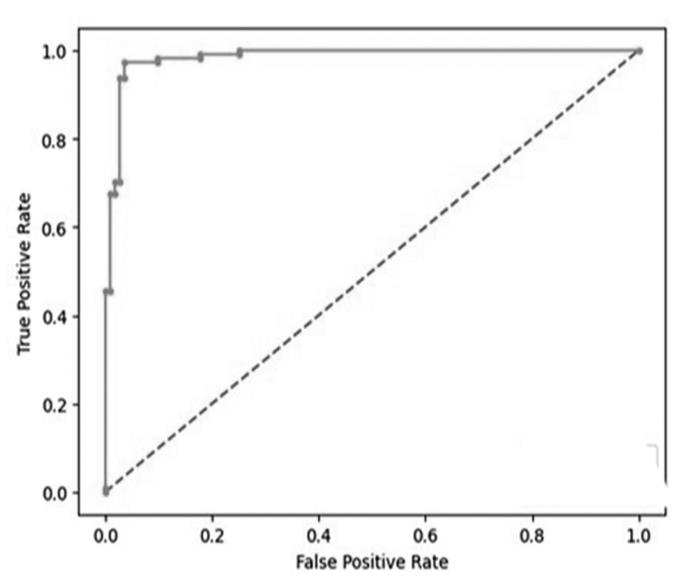
\includegraphics[width=0.95\textwidth,height=0.65\textheight,keepaspectratio]{chap5_img_12_0.png}
                
                \vspace{0.2cm}
                \textit{Hình 5.7: Biểu đồ đường cong AUROC}
            \end{center}
        \end{column}
    \end{columns}
\end{frame}

\begin{frame}{Đánh giá mô hình: Kiểm định chéo K-lần (KFCV)}
    \begin{columns}
        \begin{column}{0.4\textwidth}
            \begin{itemize}
                \item KFCV chia nhỏ dữ liệu để huấn luyện và kiểm thử chéo nhiều lần, tránh quá khớp (overfitting).
                \item Mô hình có độ chính xác rất cao và ổn định qua nhiều lần chia (K-folds).
            \end{itemize}
        \end{column}
        \begin{column}{0.6\textwidth}
            \begin{center}
                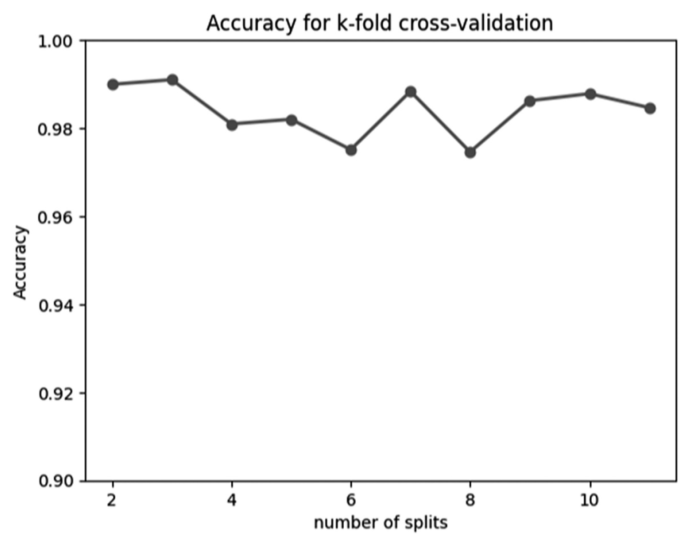
\includegraphics[width=0.95\textwidth,height=0.65\textheight,keepaspectratio]{chap5_img_13_0.png}
                
                \vspace{0.2cm}
                \textit{Hình 5.8: Độ chính xác theo số lần chia (KFCV)}
            \end{center}
        \end{column}
    \end{columns}
\end{frame}

\section{Kết luận}
\begin{frame}{Kết luận}
    \begin{itemize}
        \item Việc ứng dụng AI (đặc biệt là Học máy) vào nông nghiệp mang lại giải pháp đột phá.
        \item Hệ khuyến nghị cây trồng giúp nông dân tự tin lựa chọn giống dựa trên dữ liệu khoa học về đất đai và thời tiết thay vì kinh nghiệm truyền thống.
        \item Tối đa hóa sản lượng nông nghiệp, cải thiện thu nhập và giảm thiểu thiệt hại do biến đổi khí hậu gây ra.
    \end{itemize}
\end{frame}

\begin{frame}
    \begin{center}
        \Huge \textbf{Q \& A}
    \end{center}
\end{frame}

\end{document}
